%!TEX root = ./seminarpaper.tex

\chapter{Implemented Functions}

	This chapter gives an overview about all implemented functions. Figure \ref{fig:OverviewProbabilityDistributions} on page \pageref{fig:OverviewProbabilityDistributions} shows plots of all the distributions that have been implemented.

	\begin{figure}[h]
		\centering
		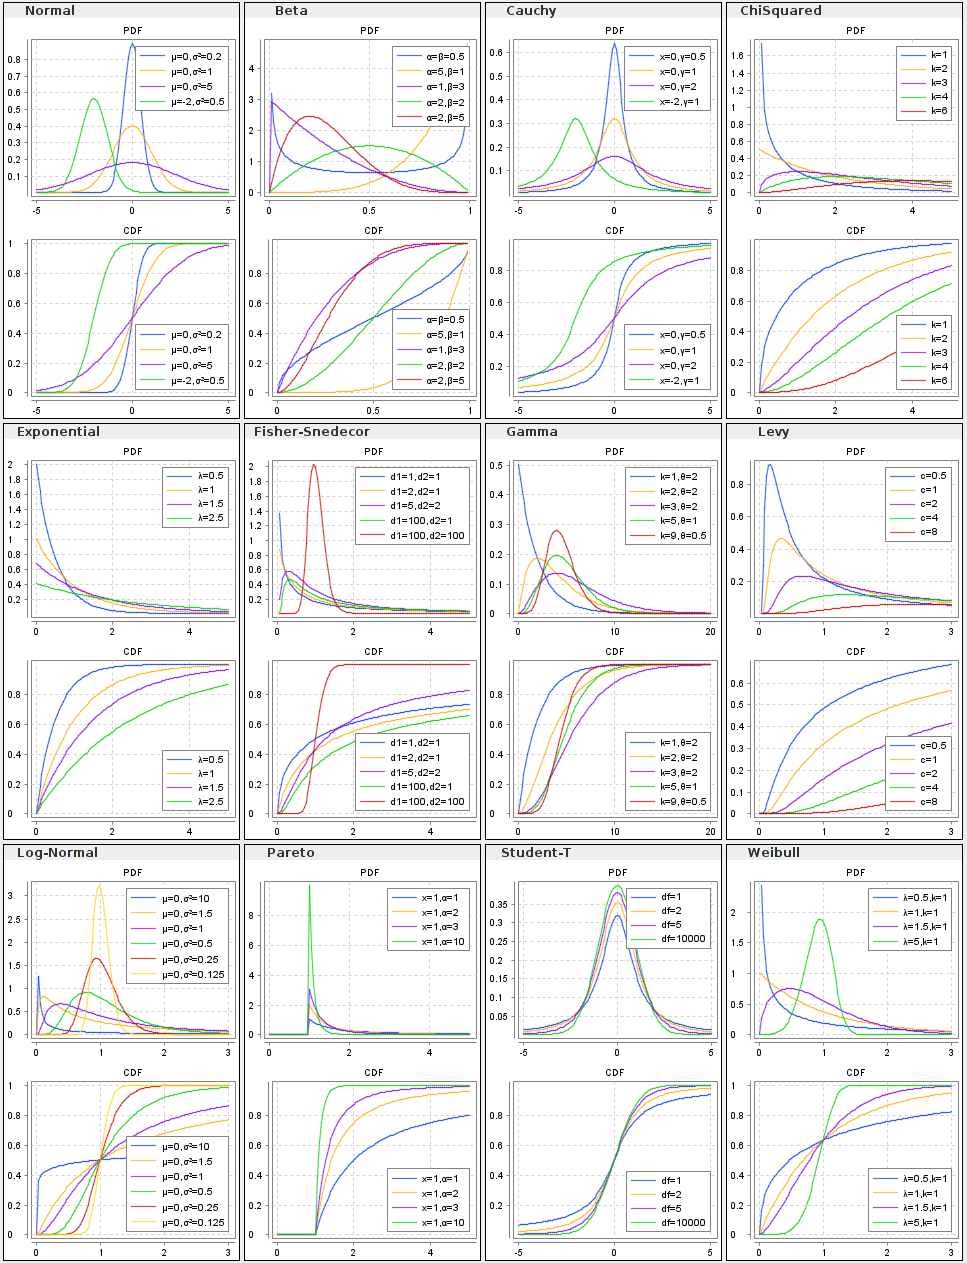
\includegraphics[width=1\textwidth]{Figures/OverviewProbabilityDistributions}~\\
		\caption{Overview Probability Distributions}
		\url{https://commons.apache.org/proper/commons-math/userguide/distribution.html}
		\label{fig:OverviewProbabilityDistributions}
	\end{figure}

	\section{Beta Distribution} \label{sec:beta_distribution}

		The \href{https://en.wikipedia.org/wiki/Beta_distribution}{Beta Distribution}\footnote{\url{https://en.wikipedia.org/wiki/Beta_distribution}} has two parameters $\alpha > 0$ and $\beta > 0$ and is defined on the interval $[0,1]$. The \ac{PDF} of the Beta Distribution is defined as

		$$f(x) = \frac{x^{\alpha-1}(1-x)^{\beta-1}}{B(\alpha,\beta)}  \hspace{.3in} 0 \le x \le 1; \alpha, \beta > 0$$
		\\[0.3cm]		
		with the beta function $B$ as a normalization constant to ensure that the total probability integrates to 1. The formula of the beta function is defined as

		$$B(\alpha,\beta) = \frac{\Gamma(\alpha)\Gamma(\beta)}{\Gamma(\alpha + \beta)}$$
		\\[0.3cm]
		where $\Gamma$ denotes the gamma function. The \ac{PDF} of the Beta Distribution is calculated in \setlx\ by calling \lstinline{stat_beta(x, alpha, beta)} or plotted on a given canvas by calling \lstinline{stat_beta_plot(alpha, beta, canvas)}.
		\\[0.3cm]		
		The \ac{CDF} of the Beta Distribution is defined as

		$$F(x) = I_{x}(\alpha,\beta) = \frac{\int_{0}^{x}{t^{\alpha-1}(1-t)^{\beta-1}dt}}{B(\alpha,\beta)} \hspace{.3in} 0 \le x \le 1; \alpha, \beta > 0$$
		\\[0.3cm]
		The \ac{CDF} of the Beta Distribution is calculated in \setlx\ by calling \lstinline{stat_betaCDF(x, alpha, beta)} or plotted on a given canvas by calling \lstinline{stat_betaCDF_plot(alpha, beta, canvas)}.


	\section{Cauchy Distribution}

		The \href{https://en.wikipedia.org/wiki/Cauchy_distribution}{Cauchy Distribution}\footnote{\url{https://en.wikipedia.org/wiki/Cauchy_distribution}} has a location parameter $t$ and a scale parameter $s$ where $s > 0$. The \ac{PDF} of the Cauchy Distribution is defined as

		$$\ds f(x) = \frac{1}{\pi} \cdot \frac{s}{s^2 + (x-t)^2} \quad \hspace{.3in} -\infty<x<\infty$$
		\\[0.3cm]
		The \ac{PDF} of the Cauchy Distribution is calculated in \setlx\ by calling \lstinline{stat_cauchy(x, t, s)} or plotted on a given canvas by calling \lstinline{stat_cauchy_plot(t, s, canvas)}.
		\\[0.3cm]
		The \ac{CDF} is defined as 

		$$\ds F(x) = \frac{1}{2} + \frac{1}{\pi} \cdot \arctan\left(\frac{x-t}{s}\right)$$
		\\[0.3cm]
		The \ac{CDF} of the Cauchy Distribution is calculated in \setlx\ by calling \lstinline{stat_cauchyCDF(x, t, s)} or plotted on a given canvas by calling \lstinline{stat_cauchyCDF_plot(t, s, canvas)}.

	\section{Chi-squared Distribution}

		The \href{https://en.wikipedia.org/wiki/Chi-squared_distribution}{Chi-squared Distribution}\footnote{\url{https://en.wikipedia.org/wiki/Chi-squared_distribution}} (also $\chi^2$-distribution) has only one parameter $k$, where $k \in \mathbb{N}_{>0}$. The \ac{PDF} of the Chi-squared Distribution is defined as

		$$f(x;\,k) =
		\begin{cases}
			\dfrac{x^{(k/2-1)} e^{-x/2}}{2^{k/2} \Gamma\left(\frac k 2 \right)},  & x > 0; \\ 0, & \text{otherwise}.
		\end{cases}$$
		\\[0.3cm]
		where $\Gamma$ is the gamma function. The \ac{PDF} of the Chi-squared Distribution is calculated in \setlx\ by calling \lstinline{stat_chiSquared(x, k)} or plotted on a given canvas by calling \lstinline{stat_chiSquared_plot(k, canvas)}.
		\\[0.3cm]
		The \ac{CDF} of the Chi-squared Distribution is defined as

		$$F(x;\,k) = \frac{\gamma(\frac{k}{2},\,\frac{x}{2})}{\Gamma(\frac{k}{2})} = P\left(\frac{k}{2},\,\frac{x}{2}\right)$$
		\\[0.3cm]
		The \ac{CDF} of the Chi-squared Distribution is calculated in \setlx\ by calling \lstinline{stat_chiSquaredCDF(x, k)} or plotted on a given canvas by calling \lstinline{stat_chiSquaredCDF_plot(k, canvas)}.

	\section{Exponential Distribution}

		The \href{https://en.wikipedia.org/wiki/Exponential_distribution}{Exponential Distribution}\footnote{\url{https://en.wikipedia.org/wiki/Exponential_distribution}} has only the parameter $\lambda$, where $\lambda > 0$. The \ac{PDF} is defined as

		$$f(x;\lambda) = \begin{cases} \lambda e^{-\lambda x} & x \ge 0, \\ 0 & x < 0. \end{cases}$$
		\\[0.3cm]
		The \ac{PDF} of the Exponential Distribution is calculated in \setlx\ by calling \lstinline{stat_exponential(x, l)} or plotted on a given canvas by calling \lstinline{stat_exponential_plot(l, canvas)}.
		\\[0.3cm]
		The \ac{CDF} is defined as

		$$F(x;\lambda) = \begin{cases} 1-e^{-\lambda x} & x \ge 0 \\ 0 & x < 0. \end{cases}$$
		\\[0.3cm]
		The \ac{CDF} of the Exponential Distribution is calculated in \setlx\ by calling \lstinline{stat_exponentialCDF(x, l)} or plotted on a given canvas by calling \lstinline{stat_exponentialCDF_plot(l, canvas)}.


	\section{Fisher-Snedecor Distribution} 

		The \href{https://en.wikipedia.org/wiki/F-distribution}{Fisher-Snedecor}\footnote{\url{https://en.wikipedia.org/wiki/F-distribution}}, or F-Distribution, has the two parameters $a$ and $b$, where $a,b \in \mathbb{N}_{>0}$. The \ac{PDF} is defined as

		$$
			f(x) = \frac{1}{\mathrm{B}\!\left(\frac{a}{2},\frac{b}{2}\right)} \left(\frac{a}{b}\right)^{\frac{a}{2}} x^{\frac{a}{2} - 1} \left(1+\frac{a}{b}\,x\right)^{-\frac{a+b}{2}}
		$$
		\\[0.3cm]
		where $\Gamma$ denotes the gamma function. The \ac{PDF} of the F-Distribution is calculated in \setlx\ by calling \lstinline{stat_fisher(x, a, b)} or plotted on a given canvas by calling \lstinline{stat_fisher_plot(a, b, canvas)}.
		\\[0.3cm]
		The \ac{CDF} is defined as

		$$F(x; a,b)=I_{\frac{a x}{a x + b}}\left (\tfrac{a}{2}, \tfrac{b}{2} \right)$$
		\\[0.3cm]
		where $I$ is the regularized incomplete beta function (see section \ref{sec:beta_distribution}). The \ac{CDF} of the F-Distribution is calculated in \setlx\ by calling \lstinline{stat_fisherCDF(x, a, b)} or plotted on a given canvas by calling \lstinline{stat_fisherCDF_plot(a, b, canvas)}.


	\section{Gamma Distribution}

		The \href{https://en.wikipedia.org/wiki/Gamma_distribution}{Gamma Distribution}\footnote{\url{https://en.wikipedia.org/wiki/Gamma_distribution}} has the shape and scale parameters $p$ and $b$, where $p,b > 0$. The \ac{PDF} is defined as

		$$f(x;p,b) =  \frac{x^{p-1}e^{-\frac{x}{b}}}{b^p\Gamma(p)} \quad \text{ for } x > 0 \text{ and } p, b > 0.$$
		\\[0.3cm]
		where $\Gamma(p)$ is a complete \href{https://en.wikipedia.org/wiki/Gamma_function}{gamma function}. The \ac{PDF} of the Gamma Distribution is calculated in \setlx\ by calling \lstinline{stat_gamma(x, p, b)} or plotted on a given canvas by calling \lstinline{stat_gamma_plot(p, b, canvas)}.
		\\[0.3cm]
		The \ac{CDF} is defined as

		$$F(x;p,b) = \int_0^x f(u;p,b)\,du = \frac{\gamma\left(p, \frac{x}{b}\right)}{\Gamma(p)}$$
		\\[0.3cm]
		where $\gamma\left(p, \frac{x}{b}\right)$ is the lower \href{https://en.wikipedia.org/wiki/Incomplete_gamma_function}{incomplete gamma function}. The \ac{CDF} of the Gamma Distribution is calculated in \setlx\ by calling \lstinline{stat_gammaCDF(x, p, b)} or plotted on a given canvas by calling \lstinline{stat_gammaCDF_plot(p, b, canvas)}.


	\section{Levy Distribution}
	
		The \href{https://en.wikipedia.org/wiki/Gamma_distribution}{Levy Distribution}\footnote{\url{https://en.wikipedia.org/wiki/Gamma_distribution}} has two parameters $\mu$ and $c$ (scale) $>$ 0 and is defined for $x \geq \mu$. The \ac{PDF} of the Levy Distribution is defined as
		\\[0.3cm]
		$$f(x;\mu,c)=\sqrt{\frac{c}{2\pi}}~~\frac{e^{ -\frac{c}{2(x-\mu)}}} {(x-\mu)^{3/2}}$$
		\\[0.3cm]
		The \ac{PDF} of the Levy Distribution is calculated in \setlx\ by calling \lstinline{stat_levy(x, mu, scale)} or plotted on a given canvas by calling \lstinline{stat_levy_plot(mu, scale, canvas)}.
		\\[0.3cm]
		The \ac{CDF} of the Levy Distribution is defined as
		\\[0.3cm]
		$$F(x;\mu,c)=\textrm{erfc}\left(\sqrt{\frac{c}{2(x-\mu)}}\right)$$
		\\[0.3cm]
		The \ac{CDF} of the Levy Distribution is calculated in \setlx\ by calling \lstinline{stat_levyCDF(x, mu, scale)} or plotted on a given canvas by calling \lstinline{stat_levyCDF_plot(mu, scale, canvas)}.

	\section{Log-Normal Distribution}
	
		The \href{https://en.wikipedia.org/wiki/Log-normal_distribution}{Log-Normal Distribution}\footnote{\url{https://en.wikipedia.org/wiki/Log-normal_distribution}} has two parameters $\mu$ (mean) and $\sigma$ (standard deviation) $>$ 0 and is defined for $x \geq 0$. The \ac{PDF} of the Log-Normal Distribution is defined as
		\\[0.3cm]
		$$f_X(x) = \frac 1 x \cdot \frac 1 {\sigma\sqrt{2\pi\,}} \exp\left( -\frac{(\ln x-\mu)^2}{2\sigma^2} \right)$$
		\\[0.3cm]
		The \ac{PDF} of the Log-Normal Distribution is calculated in \setlx\ by calling \lstinline{stat_logNormal(x, mu, sigma)} or plotted on a given canvas by calling \lstinline{stat_logNormal_plot(mu, sigma, canvas)}.
		\\[0.3cm]
		The \ac{CDF} of the Log-Normal Distribution is defined as
		\\[0.3cm]
		$$F_X(x) = \Phi\left( \frac{(\ln x) - \mu} \sigma \right)$$
		\\[0.3cm]
		The \ac{CDF} of the Log-Normal Distribution is calculated in \setlx\ by calling \lstinline{stat_logNormalCDF(x, mu, sigma)} or plotted on a given canvas by calling \lstinline{stat_logNormalCDF_plot(mu, sigma, canvas)}.

	\section{Normal Distribution}
	
		The \href{https://en.wikipedia.org/wiki/Normal_distribution}{Normal Distribution}\footnote{\url{https://en.wikipedia.org/wiki/Normal_distribution}} has two parameters $\mu$ (mean) and $\sigma$ (standard deviation) $>$ 0. The \ac{PDF} of the Normal Distribution is defined as
		\\[0.3cm]
		$$f(x \mid \mu, \sigma^2) =\frac 1 \sigma \varphi\left(\frac{x-\mu} \sigma \right)$$
		\\[0.3cm]
		The \ac{PDF} of the Normal Distribution is calculated in \setlx\ by calling \lstinline{stat_normal(x, mu, sigma)} or plotted on a given canvas by calling \lstinline{stat_normal_plot(mu, sigma, canvas)}.
		\\[0.3cm]
		The \ac{CDF} of the Normal Distribution is defined as
		\\[0.3cm]
		$$\Phi(x) = \frac 1 {\sqrt{2\pi}} \int_{-\infty}^x e^{-t^2/2}$$
		\\[0.3cm]
		The \ac{CDF} of the Normal Distribution is calculated in \setlx\ by calling \lstinline{stat_normalCDF(x, mu, sigma)} or plotted on a given canvas by calling \lstinline{stat_normalCDF_plot(mu, sigma, canvas)}.
		
	\section{Pareto Distribution}
	
		The \href{https://en.wikipedia.org/wiki/Pareto_distribution}{Pareto Distribution}\footnote{\url{https://en.wikipedia.org/wiki/Pareto_distribution}} has two parameters $\alpha$ (shape) $>$ 0 and $x_\mathrm{m}$ (scale) $>$ 0 and is defined for $x \geq x_\mathrm{m}$. The \ac{PDF} of the Pareto Distribution is defined as
		\\[0.3cm]
		$$f_X(x)= \begin{cases} \frac{\alpha x_\mathrm{m}^\alpha}{x^{\alpha+1}} & x \ge x_\mathrm{m}, \\ 0 & x < x_\mathrm{m}. \end{cases}$$
		\\[0.3cm]
		The \ac{PDF} of the Pareto Distribution is calculated in \setlx\ by calling \lstinline{stat_pareto(x, scale, shape)} or plotted on a given canvas by calling \lstinline{stat_pareto_plot(scale, shape, canvas)}.
		\\[0.3cm]
		The \ac{CDF} of the Pareto Distribution is defined as
		\\[0.3cm]
		$$F_X(x) = \begin{cases}1-\left(\frac{x_\mathrm{m}}{x}\right)^\alpha & x \ge x_\mathrm{m}, \\0 & x < x_\mathrm{m}.\end{cases}$$
		\\[0.3cm]
		The \ac{CDF} of the Pareto Distribution is calculated in \setlx\ by calling \lstinline{stat_paretoCDF(x, scale, shape)} or plotted on a given canvas by calling \lstinline{stat_paretoCDF_plot(scale, shape, canvas)}.
		
	\section{Student-T Distribution}
	
		The \href{https://en.wikipedia.org/wiki/Student\%27s_t-distribution}{Student-T Distribution}\footnote{\url{https://en.wikipedia.org/wiki/Student\%27s_t-distribution}} has one parameter $\nu$ (degrees of freedom) $>$ 0. The \ac{PDF} of the Student-T Distribution is defined as
		\\[0.3cm]
		$$f(t) = \frac{\Gamma(\frac{\nu+1}{2})} {\sqrt{\nu\pi}\,\Gamma(\frac{\nu}{2})} \left(1+\frac{t^2}{\nu} \right)^{\!-\frac{\nu+1}{2}}$$
		\\[0.3cm]
		where $\Gamma$ is the gamma function. The \ac{PDF} of the Student-T Distribution is calculated in \setlx\ by calling \lstinline{stat_student(x, nu)} or plotted on a given canvas by calling \lstinline{stat_student_plot(nu, canvas)}.
		\\[0.3cm]
		The \ac{CDF} of the Student distribution can be written in terms of $I$, the regularized incomplete beta function. For $t > 0$
		\\[0.3cm]
		$$F(t) = \int_{-\infty}^t f(u)\,du = 1 - \tfrac{1}{2} I_{x(t)}\left(\tfrac{\nu}{2}, \tfrac{1}{2}\right)$$
		\\[0.3cm]
		where $$x(t) = \frac{\nu}{{t^2+\nu}}$$
		\\[0.3cm]
		The \ac{CDF} of the Student-T Distribution is calculated in \setlx\ by calling \lstinline{stat_studentCDF(x, nu)} or plotted on a given canvas by calling \lstinline{stat_studentCDF_plot(nu, canvas)}.
		
	\section{Weibull Distribution}
	
		The \href{https://en.wikipedia.org/wiki/Weibull_distribution}{Weibull Distribution}\footnote{\url{https://en.wikipedia.org/wiki/Weibull_distribution}} has two parameters $k$ (shape) $>$ 0 and $\gamma$ (scale) $>$ 0 and is defined for $x \geq 0$. The \ac{PDF} of the Weibull Distribution is defined as
		\\[0.3cm]
		$$f(x) = \left(\frac{k}{\gamma}\right)\left(\frac{x}{\gamma}\right)^{k-1}e^{-\left(\frac{x}{\gamma}\right)^{k}} \hspace{.3in} x \geq 0; k,\gamma > 0\\$$
		\\[0.3cm]
		The \ac{PDF} of the Weibull Distribution is calculated in \setlx\ by calling \lstinline{stat_weibull(x, shape, scale)} or plotted on a given canvas by calling \lstinline{stat_weibull_plot(shape, scale, canvas)}.
		\\[0.3cm]
		The \ac{CDF} of the Weibull Distribution is defined as
		\\[0.3cm]
		$$F(x) = 1 - e^{-(x^{\gamma})} \hspace{.3in} x \geq 0; \gamma > 0$$
		\\[0.3cm]
		The \ac{CDF} of the Weibull Distribution is calculated in \setlx\ by calling \lstinline{stat_weibullCDF(x, shape, scale)} or plotted on a given canvas by calling \lstinline{stat_weibullCDF_plot(shape, scale, canvas)}.
		